\section{Open Shops} \label{sec:8}
Recall that in a flow shop, each job must follow the same route. 
In the next section, we will also discuss job shops, where each job has its 
own predetermined fixed route. However, in practice, it is often the case that 
the route of the job is immaterial and up to the schedule to decide. The 
routes of the job are \emph{open} in this sense, and this model is called 
an open shop. But we still have the usual restrictions that each machine 
can only handle one job at a time, and two operations of the same job 
cannot be run at the same time. 

\subsection{Makespan without Preemptions} \label{subsec:8.1}
We first consider the $(O_2~||~C_{\max})$ problem where there are 
two machines. A job $j$ can be processed first on machine $1$ or 
vice versa; the decision maker can determine the routes. It is clear that 
\[ C_{\max} \geq \max\left( \sum_{j=1}^n p_{1j}, \sum_{j=1}^n p_{2j} \right), \] 
since the makespan cannot be less than the workload on either machine. 

One might expect that this is an equality, and this is true 
in most situations. However, to get equality, we must also consider 
$\max_{j\in[n]} p_{1j} + p_{2j}$ because of the restriction 
that two operations of the same job cannot be run at the same time. 
Thus, the optimal makespan is 
\[ C_{\max} = \max\left( \max_{j\in[n]} (p_{1j} + p_{2j}), 
\sum_{j=1}^n p_{1j}, \sum_{j=1}^n p_{2j} \right). \] 
For now, we only consider non-delay schedules. That is, if there is a job 
waiting for processing when a machine is free, then that machine is 
not allowed to remain idle. It follows that an idle period can occur 
on a machine if and only if one job remains to be processed on that machine 
and when that machine is available, this last job is still being processed 
on the other machine. Such an idle period \emph{can} cause an unnecessary 
increase in the makespan. If this last job turns out to be the very last 
job to complete all its processing, then the idle period does cause 
an increase in the makespan. But if this last job, after having 
completed its processing on the machine that was idle, is \emph{not} 
the very last job to leave the system, then the makespan is still 
equal to the maximum of the two workloads. 

We now give an algorithm that solves $(O_2~||~C_{\max})$ instances in 
polynomial time. We may assume without loss of generality that the 
longest processing time among the $2n$ processing times belongs to 
operation $(1, k)$, because we can swap the two machines if needed. 
That is, we have $p_{ij} \leq p_{1k}$ for all $i = 1, 2$ and 
$j = 1, \dots, n$. 

\begin{algo}{algo:8.1}
    If operation $(1, k)$ is the longest operation, then job $k$ must be 
    started at time $0$ on machine $2$.
    After job $k$ has completed its processing on machine $2$, 
    its operation $(1, k)$ has the lowest possible priority with 
    regard to processing on machine $1$. Then the processing of 
    operation $(1, k)$ will be postponed as much as possible; 
    it can only be processed on machine $1$ if no other job is 
    available for processing on machine $1$. (This can only 
    happen either if it is the last operation to be done on 
    machine $1$, or if it is the second last operation and the 
    last operation is not available because it is still being 
    processed on machine $2$.) The $2(n-1)$ operations 
    of the remaining $n-1$ jobs can be processed on the two machines 
    in any order. However, unforced idleness is not allowed. 
\end{algo} 

Algorithm~\ref{algo:8.1} is a more general form of the 
{\bf Longest Alternate Processing Time first (LAPT)} rule, which says 
that whenever a machine is freed, start processing the jobs that have 
not yet received processing on either machine the one with the longest 
processing time on the \emph{other} machine. 

\begin{theo}{theo:8.2}
    Algorithm~\ref{algo:8.1} results in an optimal schedule for 
    $(O_2~||~C_{\max})$ with makespan 
    \[ C_{\max} = \max\left( \max_{j\in[n]} (p_{1j} + p_{2j}), 
    \sum_{j=1}^n p_{1j}, \sum_{j=1}^n p_{2j} \right). \] 
\end{theo}
\begin{pf}
    If the resulting schedule has no idle period on either machine, then 
    it is of course optimal. However, an idle period may occur either on 
    machine $1$ or on machine $2$. We consider two cases. 

    {\sc Case 1.} Suppose an idle period occurs on machine $2$. 
    If this is the case, then only one more operation needs processing on 
    machine $2$ but this operation still has to complete its processing 
    on machine $1$. Assume that this operation belongs to job $\ell$. 
    When job $\ell$ starts on machine $2$, job $k$ starts on machine $1$
    and $p_{1k} > p_{2\ell}$. Hence, the makespan is determined by the 
    completion of job $k$ on machine $1$ and no idle period has occurred 
    on machine $1$. This means the schedule is optimal. 

    {\sc Case 2.} Suppose an idle period occurs on machine $1$. An idle period 
    on machine $1$ can occur only when machine $1$ is freed after completing 
    all its operations with the exception of operation $(1, k)$, and operation 
    $(2, k)$ of job $k$ is still being processed on machine $2$ at that point. 
    In this case, the makespan is equal to $p_{2k} + p_{1k}$ and the schedule 
    is optimal.
\end{pf}

The LAPT rule we described above can be considered to be a special case 
of a more general rule that can be applied to open shops with more than 
two machines. This rule is called the {\bf Longest Total Remaining 
Processing on Other Machines first (LTRPOM)} rule. According to this rule, 
the processing required on the machine currently available does not 
affect the priority level of a job. However, this rule does not always 
result in an optimal schedule because the $(O_m~||~C_{\max})$ problem is 
$\NP$-hard when $m \geq 3$. 

\begin{theo}{theo:8.3}
    The $(O_3~||~C_{\max})$ problem is weakly $\NP$-hard. 
\end{theo}
\begin{pf}
    We prove this using a reduction from {\sc Partition} to 
    $(O_3~||~C_{\max})$. Given $a_1, \dots, a_t, b \in \Z^+$ such that 
    $\sum_{j=1}^t a_j = 2b$, we construct $n = 3t + 1$ jobs. There are three 
    jobs corresponding to each value $a_j$, given by 
    \begin{align*}
        p_{1j} &= a_j, & p_{2j} &= 0, & p_{3j} &= 0, & j &= 1, \dots, t, \\
        p_{1j} &= 0, & p_{2j} &= a_j, & p_{3j} &= 0, & j &= t+1, \dots, 2t, \\
        p_{1j} &= 0, & p_{2j} &= 0, & p_{3j} &= a_j, & j &= 2t+1, \dots, 3t.
    \end{align*}
    There is one more marker job with processing times 
    \[ p_{1,3t+1} = p_{2,3t+1} = p_{3,3t+1} = b. \] 
    Let $z^* = 3b$. We claim that there is a schedule with makespan 
    $z^*$ if and the {\sc Partition} instance has a solution. 
    Suppose there is a schedule with makespan $z^* = 3b$. Assume 
    without loss of generality that the marker job $3t+1$ is scheduled 
    on time interval $[b, 2b]$ on machine $1$, because we could swap 
    machines otherwise. Then the jobs processed at time interval 
    $[0, b]$ on machine $1$ correspond to a subset $S_1 \subseteq 
    \{1, \dots, t\}$ such that $\sum_{j\in S_1} a_j = b$, 
    as do the jobs processed at time interval $[2b, 3b]$ on machine $2$. 
    Thus, the {\sc Partition} instance has a solution. 
 
    Suppose that the {\sc Partition} instance has a solution, namely a 
    partition $(S_1, S_2)$ of $\{1, \dots, t\}$ such that 
    $\sum_{j\in S_1} a_j = \sum_{j\in S_2} a_j = b$. Process 
    job $3t+1$ on machine $2$ at time interval $[0, b]$, on machine 
    $1$ at time interval $[b, 2b]$, and on machine $3$ at time interval 
    $[2b, 3b]$. Then we could place all jobs in $S_1$ on machine $1$ 
    at time interval $[0, b]$ and all jobs in $S_2$ on machine $1$ 
    at time interval $[2b, 3b]$. This will extend naturally to a schedule 
    with makespan $z^* = 3b$. 
\end{pf}

The schedule from the proof of Theorem~\ref{theo:8.3} is described 
in the following Gantt chart. 
\begin{center}
    \begin{tikzpicture}[/pgfgantt/y unit chart=0.65cm] 
        \begin{ganttchart}[
            title/.style={draw=none},
            canvas/.append style={draw=none}, 
            bar top shift=0.1, bar height=0.6,
            y unit title=0.65cm,
        ]{1}{15}
            \ganttbar{Machine 1}{1}{5} \ganttbar[inline]{}{1}{5} \ganttbar[inline, bar/.append style={fill=gray}]{Job $3t+1$}{6}{10} \ganttbar[inline]{}{11}{15} \\ 
            \ganttbar{Machine 2}{1}{5} \ganttbar[inline, bar/.append style={fill=gray}]{Job $3t+1$}{1}{5} \ganttbar[inline]{}{6}{10} \ganttbar[inline]{}{11}{15} \\ 
            \ganttbar{Machine 3}{1}{5} \ganttbar[inline]{}{1}{5} \ganttbar[inline]{}{6}{10} \ganttbar[inline, bar/.append style={fill=gray}]{Job $3t+1$}{11}{15} \\ 
            \ganttbar[inline, bar/.style={draw=none}]{$b$}{5}{5} \ganttbar[inline, bar/.style={draw=none}]{$2b$}{10}{10} \ganttbar[inline, bar/.style={draw=none}]{$3b$}{15}{15}
        \end{ganttchart}
    \end{tikzpicture}
\end{center}   
\vspace{-0.4cm}
Algorithm~\ref{algo:8.1} is one of the few polynomial time algorithms 
for non-preemptive open shop problems. Most of the more general open shop 
models are $\NP$-hard, such as $(O_2~|~r_j~|~C_{\max})$. However, it turns 
out that the problem $(O_m~|~r_j, p_{ij} = 1~|~C_{\max})$ can be solved 
in polynomial time. We discuss this further in Section~\ref{subsec:8.3}. 

\subsection{Makespan with Preemptions} \label{subsec:8.2} 
Preemptive open shop problems tend to be somewhat easier. In contrast 
to the $(O_m~||~C_{\max})$ problem, we will see that the 
$(O_m~|~\text{prmp}~|~C_{\max})$ problem is solvable in polynomial time. 

Note that the value of the makespan under Algorithm~\ref{algo:8.1} 
(or LAPT) is a lower bound for the makespan with two machines, 
even when preemptions are allowed. It follows that these non-preemptive 
rules are also optimal for $(O_2~|~\text{prmp}~|~C_{\max})$. 

An easy lower bound for the makespan with $m \geq 3$ machines when 
preemptions are allowed is 
\[ C_{\max} \geq \max \left( \max_{j\in[n]} \sum_{i=1}^m p_{ij},\; 
\max_{i\in[m]} \sum_{j=1}^n p_{ij} \right). \] 
That is, the makespan must be at least as large as the maximum workload 
on each of the $m$ machines, and at least as large as the total amount 
of processing to be done on each of the $n$ jobs. It turns out that 
it is not difficult to obtain a schedule whose makespan is equal to this 
lower bound. To see how this is done, we define 
\[ \text{ML}_i = \sum_{j=1}^n p_{ij} \] 
for each $i = 1, \dots, m$ to be the load of machine $i$, and 
\[ \text{JL}_j = \sum_{i=1}^m p_{ij} \] 
for each $j = 1, \dots, n$ to be the load of job $j$. 
We can view these as the sums of the rows and columns of the 
the $m \times n$ matrix $\mathbf P$ corresponding to the processing times
$p_{ij}$. Let $\text{LB}$ be the lower bound from above. 

We call machine $i$ {\bf tight} if we have $\text{ML}_i = \text{LB}$. 
Similarly, we call job $j$ {\bf tight} if $\text{JL}_j = \text{LB}$. 
If machine $i$ or job $j$ are not tight, then they have {\bf slack}. 
A set $D$ of operations is called a {\bf decrementing set} if it contains 
one entry for each tight job, one entry for each tight machine, 
and at most one entry for each slack row and slack column. 
Similar to the matrix $\mathbf P$ of processing times, this set $D$ can be 
viewed as an $m \times n$ matrix consisting of entries from $\{0, 1\}$. 

\begin{theo}{theo:8.4}
    A decrementing set always exists and can be computed in polynomial time.
\end{theo}

We take this result for granted, but note that the proof is based on 
maximal cardinality matchings. We can use a decrementing set to 
construct a partial schedule of length $\Delta$ for some appropriately 
chosen $\Delta$. We are now ready to state the algorithm for 
$(O_m~|~\text{prmp}~|~C_{\max})$, which, finds a schedule 
with makespan $C_{\max} = \text{LB}$.

\begin{algo}{algo:8.5}
    Repeat the following steps until all operations have been successfully scheduled.
    \begin{enumerate}[(1)]
        \item Find a decrementing set $D$. 
        \item Find the maximum value of $\Delta$ such that 
        \begin{enumerate}[(i)]
            \item $\Delta \leq \min_{(i,j) \in D} p_{ij}$;
            \item $\Delta \leq \text{LB} - \text{ML}_i$ if machine $i$ 
            has slack and no operation in $D$; 
            \item $\Delta \leq \text{LB} - \text{JL}_j$ if job $j$ 
            has slack and no operation in $D$. 
        \end{enumerate}
        \item Schedule the operations in $D$ for $\Delta$ time units 
        in parallel. 
        \item Update the values of $p_{ij}$, $\text{LB}$, $\text{ML}_i$, 
        and $\text{JL}_j$. 
    \end{enumerate}
\end{algo}

Note that after each iteration, we are decreasing LB by $\Delta$, 
and a slice of $\Delta$ time units is scheduled. This suggests that 
the algorithm terminates after $\leq \text{LB}$ iterations. But we can actually 
do a slightly better analysis than this: it terminates after $\leq nm + n + m$ 
iterations. To see why, observe that at each iteration, either 
\begin{itemize}
    \item an operation gets completely scheduled, or 
    \item a slack machine or job becomes tight (and stays tight throughout 
    the later iterations).
\end{itemize}
In particular, the algorithm is polynomial time and is correct.  

\begin{exmp}{exmp:8.6}
    Consider $3$ machines and $4$ jobs with the processing times being 
    the entries in the matrix 
    \[ \mathbf P = \begin{bmatrix}
        3 & 4 & 0 & 4 \\ 
        4 & 0 & 6 & 0 \\ 
        4 & 0 & 0 & 6
    \end{bmatrix}. \] 
    We can easily see that $\text{LB} = 11$ by computing the sums of the 
    rows and columns. In particular, observe that machine $1$ 
    and job $1$ are tight, while all other machines and jobs are slack. One 
    possible decrementing set comprises of the processing times 
    $p_{12} = 4$, $p_{21} = 4$, and $p_{34} = 6$. We can choose 
    $\Delta = 4$ in this case, and a partial schedule is constructed 
    by scheduling job $2$ on machine $1$ for $4$ time units, 
    job $1$ on machine $2$ for $4$ time units, and 
    job $4$ on machine $3$ for $4$ time units. The matrix is now 
    \[ \mathbf P = \begin{bmatrix}
        3 & 0 & 0 & 4 \\ 
        0 & 0 & 6 & 0 \\ 
        4 & 0 & 0 & 2
    \end{bmatrix}, \] 
    and $\text{LB} = 7$. This means that machine $1$ and job $1$ are again 
    tight, with all other machines and jobs being slack. A decrementing set 
    is obtained with the processing times $p_{14} = 4$, $p_{23} = 6$, 
    and $p_{41} = 4$. Then for $\Delta = 4$, we can augment the partial 
    schedule by assigning job $4$ to machine $1$ for $4$ time units, 
    job $3$ to machine $2$ for $4$ time units, and job $1$ to machine $3$ 
    for $4$ time units. The matrix is updated to 
    \[ \mathbf P = \begin{bmatrix}
        3 & 0 & 0 & 0 \\ 
        0 & 0 & 2 & 0 \\ 
        0 & 0 & 0 & 2
    \end{bmatrix}. \] 
    At this point, there is an obvious way to assign the remaining 
    processing times. We can put job $1$ on machine $1$ for $3$ time units, 
    job $3$ on machine $2$ for $2$ time units, and job $4$ on machine $3$ 
    for $2$ time units.
\end{exmp}

The schedule from Example~\ref{exmp:8.6} is depicted in the following Gantt chart.
\begin{center}
    \begin{tikzpicture}[/pgfgantt/y unit chart=0.65cm] 
        \begin{ganttchart}[
            title/.style={draw=none},
            canvas/.append style={draw=none}, 
            bar top shift=0.1, bar height=0.6,
            y unit title=0.65cm,
        ]{1}{11}
            \ganttbar{Machine 1}{1}{4} \ganttbar[inline]{2}{1}{4} \ganttbar[inline]{4}{5}{8} \ganttbar[inline]{1}{9}{11} \\ 
            \ganttbar{Machine 2}{1}{4} \ganttbar[inline]{1}{1}{4} \ganttbar[inline]{3}{5}{8} \ganttbar[inline]{3}{9}{10} \\ 
            \ganttbar{Machine 3}{1}{4} \ganttbar[inline]{4}{1}{4} \ganttbar[inline]{1}{5}{8} \ganttbar[inline]{4}{9}{10} \\ 
            \gantttitlelist{1,...,11}{1}
        \end{ganttchart}
    \end{tikzpicture}
\end{center}   
\vspace{-0.4cm}

\subsection{Maximum Lateness without Preemptions} \label{subsec:8.3} 
The $(O_m~||~L_{\max})$ problem is a generalization of the 
$(O_m~||~C_{\max})$ problem, and is therefore at least as hard. 

\begin{theo}{theo:8.7}
    The problem $(O_2~||~L_{\max})$ is strongly $\NP$-hard.
\end{theo}
\begin{pf}
    We reduce \textsc{$3$-Partition} to $(O_2~||~L_{\max})$. Given 
    $a_1, \dots, a_{3t}, b \in \Z^+$ under the usual assumptions, we 
    construct $n = 4t$ jobs with processing times 
    \begin{align*}
        p_{1j} &= 0, & p_{2j} &= a_j, & d_j &= 3tb, & j &= 1, \dots, 3t, \\ 
        p_{1j} &= 0, & p_{2j} &= 2b, & d_j &= 2b, & j &= 3t+1, \\ 
        p_{1j} &= 3b, & p_{2j} &= 2b, & d_j &= (3(j-3t)-1)b, & j &= 3t+2, \dots, 4t.
    \end{align*}
    In particular, jobs $3t+1, \dots, 4t$ are marker jobs, with the 
    last job having due date $(3t-1)b$. Then there exists a schedule 
    with $L_{\max} \leq 0$ if and only if jobs $1, \dots, 3t$ can be 
    divided into $t$ groups, each containing three jobs and requiring 
    $b$ units of processing time on machine $2$. This is equivalent to 
    the \textsc{$3$-Partition} instance having a solution. 
\end{pf}

We can show that $(O_2~||~L_{\max})$ is equivalent to the 
$(O_2~|~r_j~|~C_{\max})$ problem. Indeed, consider the $(O_2~||~L_{\max})$ 
problem with deadlines $\overline{d_j}$ rather than due dates $d_j$. 
Let 
\[ \overline{d_{\max}} = \max_{j\in [n]} \overline{d_j}. \] 
Applying a time reversal to $(O_2~||~L_{\max})$, we see that finding a 
feasible schedule with $L_{\max} = 0$ is now equivalent to finding 
a schedule for $(O_2~|~r_j~|~C_{\max})$ with release dates 
\[ r_j = \overline{d_{\max}} - \overline{d_j} \] 
and a makespan that is less than $\overline{d_{\max}}$. Thus, the 
$(O_2~|~r_j~|~C_{\max})$ problem is also strongly $\NP$-hard. 

Now, we consider the special case $(O_m~|~r_j, p_{ij} = 1~|~L_{\max})$ 
that we mentioned at the end of Section~\ref{subsec:8.1}. The fact that 
all the processing times are unit makes the problem considerably easier. 
The polynomial time solution procedure consists of three phases. 
\begin{itemize}
    \item {\bf Phase 1:} Parametrizing and a binary search. 
    \item {\bf Phase 2:} Solving a network flow problem. 
    \item {\bf Phase 3:} Colouring a bipartite graph.  
\end{itemize}
At Phase 1, we let $L$ be a free parameter and assume that each job has a 
deadline $d_j + L$. The objective is to find a schedule in which each job 
is completed by its deadline, ensuring that $L_{\max} \leq L$. We set 
\[ t_{\max} = \max(d_1, \dots, d_n) + L. \] 
That is, no job should receive any processing after time $t_{\max}$. 

Phase 2 focuses on the following network flow problem. There is a source 
node $U$ that has $n$ arcs going to nodes $1, \dots, n$, where node $j$ 
corresponds to job $j$. The arc from the source node $U$ to node $j$ 
has capacity $m$, which is equal to the number of machines and the number 
of operations on each job. There is a second set of $t_{\max}$ nodes, 
with each node corresponding to one time unit. A node $t$ with 
$t = 1, \dots, t_{\max}$ represents the time slot $[t-1, t]$. A node $j$ 
has arcs going to nodes $r_j + 1, \dots, d_j + L$, and these arcs have 
unit capacity. Finally, each node in the set of $t_{\max}$ nodes 
has an arc of capacity $m$ going to the sink node $V$. This capacity limit 
ensures that no more than $m$ operations are processed in any given time 
period. The solution of this network flow problem indicates which time 
slots the $m$ operations of job $j$ need to be processed in. 
\begin{center}
    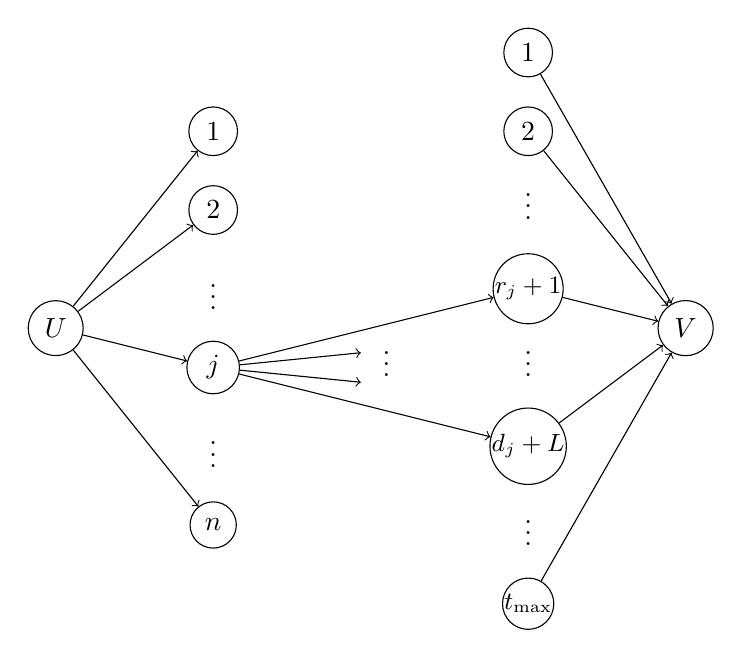
\begin{tikzpicture}              
        \node [circle, draw=black] (U) at (0, 5) {$U$};

        \node [circle, draw=black] (J1) at (2, 7.5) {$1$};
        \node [circle, draw=black] (J2) at (2, 6.5) {$2$};
        \node (Jdots1) at (2, 5.5) {$\vdots$};
        \node [circle, draw=black] (Jj) at (2, 4.5) {$j$};
        \node (Jdots2) at (2, 3.5) {$\vdots$};
        \node [circle, draw=black] (Jn) at (2, 2.5) {$n$};

        \node (blank) at (4, 4.7) {};
        \node (blank2) at (4, 4.3) {};
        \node (dots) at (4.2, 4.65) {$\vdots$};

        \node [circle, draw=black] (T1) at (6, 8.5) {$1$};
        \node [circle, draw=black] (T2) at (6, 7.5) {$2$};
        \node (Tdots1) at (6, 6.65) {$\vdots$};
        \node [circle, draw=black, inner sep=0pt, minimum size=1pt] (Trj) at (6, 5.5) {\small $r_j+1$ \normalsize};
        \node (Tdots2) at (6, 4.65) {$\vdots$};
        \node [circle, draw=black, inner sep=0pt, minimum size=1pt] (Tdj) at (6, 3.5) {\small $d_j+L$ \normalsize};
        \node (Tdots3) at (6, 2.5) {$\vdots$};
        \node [circle, draw=black, inner sep=0pt, minimum size=1pt] (Ttmax) at (6, 1.5) {\small $t_{\max}$ \normalsize};

        \node [circle, draw=black] (V) at (8, 5) {$V$};
        
        \draw [->] (U) -- (J1); \draw [->] (U) -- (J2); \draw [->] (U) -- (Jj); \draw [->] (U) -- (Jn);
        \draw [->] (T1) -- (V); \draw [->] (T2) -- (V); \draw [->] (Trj) -- (V); \draw [->] (Tdj) -- (V); \draw [->] (Ttmax) -- (V);
        \draw [->] (Jj) -- (Trj); \draw [->] (Jj) -- (Tdj);
        \draw [->] (Jj) -- (blank); \draw [->] (Jj) -- (blank2);
    \end{tikzpicture} 
\end{center}
One can also consider this network flow problem as a transportation model with 
\begin{align*}
    \min\quad & 0 \\ 
    \text{s.t.}\quad & \sum_{t=r_j+1}^{d_j+L} x_{jt} = m, && j = 1, \dots, n, \\ 
    & \sum_{j=1}^n x_{jt} \leq m, && t = 1, \dots, t_{\max}, \\ 
    & x_{jt} \leq 1, && j = 1, \dots, n,\; t = 1, \dots, t_{\max}, \\ 
    & x_{jt} \geq 0, && j = 1, \dots, n,\; t = 1, \dots, t_{\max}. 
\end{align*}
The first set of constraints ensures that for each job, all operations are 
run and are timely. The second set of constraints ensures that each time unit 
can only process at most $m$ jobs, corresponding to the number of machines. 
Note that the objective value is arbitrary here because all we need is a 
feasible solution. We recall that the unimodularity property ensures that 
an optimal solution is integer, and that such an LP can be solved in 
polynomial time. 

However, the solution to the network flow problem cannot be immediately 
translated into a feasible schedule for the open shop, because in the 
network flow formulation, no distinction is made between the different 
machines. But we can transform the assignment of operations to time slots 
prescribed by the network flow solution into a feasible schedule in 
such a way that every job $j$ is processed on a different machine 
at each time unit. 

Phase 3 of the algorithm generates a feasible schedule. From the 
solution of the network flow problem, we can construct a bipartite graph 
with two sets $N_1$ and $N_2$ of nodes. The set $N_1$ has $n$ nodes 
corresponding to the jobs, and $N_2$ has $t_{\max}$ nodes corresponding 
to the time slots. A node in $N_1$ is connected to the $m$ nodes in 
$N_2$ corresponding to the time slots in which its operations 
are supposed to be processed, prescribed by the solution from Phase 2. 
So each node in $N_1$ is connected to exactly $m$ nodes in $N_2$, 
while each node in $N_2$ is connected to at most $m$ nodes in $N_1$. 
A result in graph theory tells us that if each node in a bipartite graph 
has at most $m$ arcs, then the arcs can be coloured with $m$ different 
colours in such a way that no node has two arcs of the same colour. 
Each colour then corresponds to a machine. 

The colouring algorithm is fairly straightforward and was covered in 
MATH 239. Find a matching in the bipartite graph and colour all the 
edges in that matching with the same colour. Remove that matching 
from the graph and repeat this procedure until all edges have been coloured. 

\begin{exmp}{exmp:8.8}
    Consider the following instance of $(O_3~|~r_j, p_{ij} = 1~|~L_{\max})$ 
    with $3$ machines and $7$ jobs. 
    \begin{align*}
        \begin{array}{c|ccccccc}
            \text{Jobs} & 1 & 2 & 3 & 4 & 5 & 6 & 7 \\ \hline 
            r_j & 0 & 1 & 2 & 2 & 3 & 4 & 5 \\ 
            d_j & 5 & 5 & 5 & 6 & 6 & 8 & 8
        \end{array}
    \end{align*}
    Assume that $L = 1$. Each job has a deadline $\overline{d_j} = d_j + 1$, 
    and we have $t_{\max} = 9$. In Phase 2, we have the network flow 
    problem described below. 
    \begin{center}
        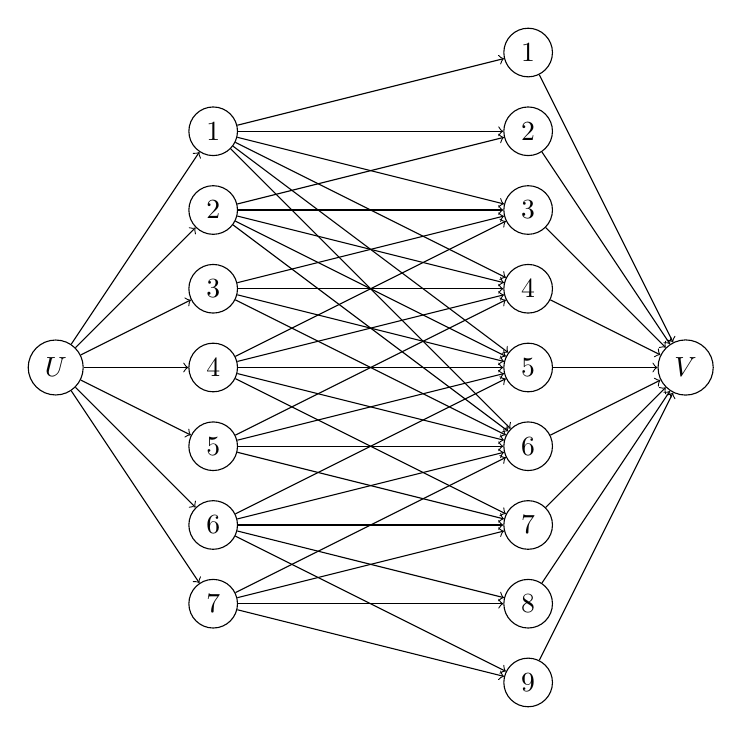
\begin{tikzpicture}              
            \node [circle, draw=black] (U) at (0, 5) {$U$};
    
            \node [circle, draw=black] (J1) at (2, 8) {$1$};
            \node [circle, draw=black] (J2) at (2, 7) {$2$};
            \node [circle, draw=black] (J3) at (2, 6) {$3$};
            \node [circle, draw=black] (J4) at (2, 5) {$4$};
            \node [circle, draw=black] (J5) at (2, 4) {$5$};
            \node [circle, draw=black] (J6) at (2, 3) {$6$};
            \node [circle, draw=black] (J7) at (2, 2) {$7$};
    
            \node [circle, draw=black] (T1) at (6, 9) {$1$};
            \node [circle, draw=black] (T2) at (6, 8) {$2$};
            \node [circle, draw=black] (T3) at (6, 7) {$3$};
            \node [circle, draw=black] (T4) at (6, 6) {$4$};
            \node [circle, draw=black] (T5) at (6, 5) {$5$};
            \node [circle, draw=black] (T6) at (6, 4) {$6$};
            \node [circle, draw=black] (T7) at (6, 3) {$7$};
            \node [circle, draw=black] (T8) at (6, 2) {$8$};
            \node [circle, draw=black] (T9) at (6, 1) {$9$};
    
            \node [circle, draw=black] (V) at (8, 5) {$V$};
            
            \draw [->] (U) -- (J1); \draw [->] (U) -- (J2); \draw [->] (U) -- (J3);
            \draw [->] (U) -- (J4); \draw [->] (U) -- (J5); \draw [->] (U) -- (J6);
            \draw [->] (U) -- (J7); 


            \draw [->] (T1) -- (V); \draw [->] (T2) -- (V); \draw [->] (T3) -- (V);
            \draw [->] (T4) -- (V); \draw [->] (T5) -- (V); \draw [->] (T6) -- (V);
            \draw [->] (T7) -- (V); \draw [->] (T8) -- (V); \draw [->] (T9) -- (V);

            \draw [->] (J1) -- (T1); \draw [->] (J1) -- (T2); \draw [->] (J1) -- (T3);
            \draw [->] (J1) -- (T4); \draw [->] (J1) -- (T5); \draw [->] (J1) -- (T6);

            \draw [->] (J2) -- (T2); \draw [->] (J2) -- (T3); \draw [->] (J2) -- (T4); 
            \draw [->] (J2) -- (T5); \draw [->] (J2) -- (T6);

            \draw [->] (J3) -- (T3); \draw [->] (J3) -- (T4); 
            \draw [->] (J3) -- (T5); \draw [->] (J3) -- (T6);

            \draw [->] (J4) -- (T3); \draw [->] (J4) -- (T4); 
            \draw [->] (J4) -- (T5); \draw [->] (J4) -- (T6); \draw [->] (J4) -- (T7);

            \draw [->] (J5) -- (T4); \draw [->] (J5) -- (T5); 
            \draw [->] (J5) -- (T6); \draw [->] (J5) -- (T7);

            \draw [->] (J6) -- (T5); \draw [->] (J6) -- (T6); \draw [->] (J6) -- (T7);
            \draw [->] (J6) -- (T8); \draw [->] (J6) -- (T9);

            \draw [->] (J7) -- (T6); \draw [->] (J7) -- (T7);
            \draw [->] (J7) -- (T8); \draw [->] (J7) -- (T9);
        \end{tikzpicture} 
    \end{center}
    Solving this network flow problem, we see that the jobs can be 
    processed during the time units in the following table. 
    \begin{align*}
        \begin{array}{c|ccccccc}
            \text{Jobs} & 1 & 2 & 3 & 4 & 5 & 6 & 7 \\ \hline 
            \text{Time Units} & 1, 2, 3 & 2, 3, 4 & 4, 5, 6 & 4, 5, 6 & 5, 6, 7 & 7, 8, 9 & 7, 8, 9
        \end{array}
    \end{align*}
    It is not hard to verify that at most three jobs are processed 
    simultaneously for any given point in time. 

    Phase 3 leads to the graph colouring problem for the following 
    bipartite graph. 
    \begin{center}
        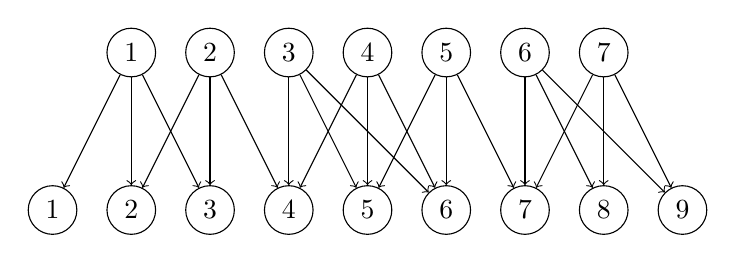
\begin{tikzpicture}              
            \node [circle, draw=black] (J1) at (3, 6) {$1$}; 
            \node [circle, draw=black] (J2) at (4, 6) {$2$}; 
            \node [circle, draw=black] (J3) at (5, 6) {$3$}; 
            \node [circle, draw=black] (J4) at (6, 6) {$4$}; 
            \node [circle, draw=black] (J5) at (7, 6) {$5$}; 
            \node [circle, draw=black] (J6) at (8, 6) {$6$}; 
            \node [circle, draw=black] (J7) at (9, 6) {$7$}; 
            
            \node [circle, draw=black] (T1) at (2, 4) {$1$}; 
            \node [circle, draw=black] (T2) at (3, 4) {$2$}; 
            \node [circle, draw=black] (T3) at (4, 4) {$3$}; 
            \node [circle, draw=black] (T4) at (5, 4) {$4$}; 
            \node [circle, draw=black] (T5) at (6, 4) {$5$}; 
            \node [circle, draw=black] (T6) at (7, 4) {$6$}; 
            \node [circle, draw=black] (T7) at (8, 4) {$7$}; 
            \node [circle, draw=black] (T8) at (9, 4) {$8$}; 
            \node [circle, draw=black] (T9) at (10, 4) {$9$};
            
            \draw [->] (J1) -- (T1); \draw [->] (J1) -- (T2); \draw [->] (J1) -- (T3); 
            \draw [->] (J2) -- (T2); \draw [->] (J2) -- (T3); \draw [->] (J2) -- (T4); 
            \draw [->] (J3) -- (T4); \draw [->] (J3) -- (T5); \draw [->] (J3) -- (T6);
            \draw [->] (J4) -- (T4); \draw [->] (J4) -- (T5); \draw [->] (J4) -- (T6); 
            \draw [->] (J5) -- (T5); \draw [->] (J5) -- (T6); \draw [->] (J5) -- (T7); 
            \draw [->] (J6) -- (T7); \draw [->] (J6) -- (T8); \draw [->] (J6) -- (T9); 
            \draw [->] (J7) -- (T7); \draw [->] (J7) -- (T8); \draw [->] (J7) -- (T9); 
        \end{tikzpicture} 
    \end{center}
    We find matchings and remove them until all edges are coloured. 
    \begin{center}
        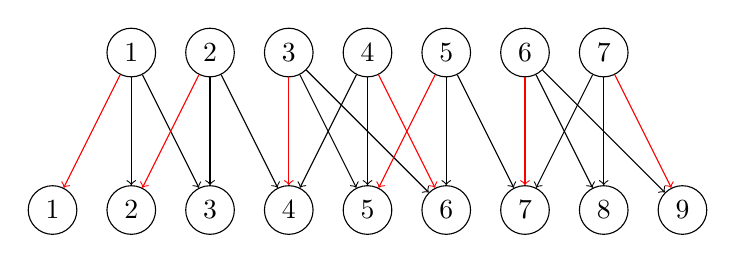
\begin{tikzpicture}              
            \node [circle, draw=black] (J1) at (3, 6) {$1$}; 
            \node [circle, draw=black] (J2) at (4, 6) {$2$}; 
            \node [circle, draw=black] (J3) at (5, 6) {$3$}; 
            \node [circle, draw=black] (J4) at (6, 6) {$4$}; 
            \node [circle, draw=black] (J5) at (7, 6) {$5$}; 
            \node [circle, draw=black] (J6) at (8, 6) {$6$}; 
            \node [circle, draw=black] (J7) at (9, 6) {$7$}; 
            
            \node [circle, draw=black] (T1) at (2, 4) {$1$}; 
            \node [circle, draw=black] (T2) at (3, 4) {$2$}; 
            \node [circle, draw=black] (T3) at (4, 4) {$3$}; 
            \node [circle, draw=black] (T4) at (5, 4) {$4$}; 
            \node [circle, draw=black] (T5) at (6, 4) {$5$}; 
            \node [circle, draw=black] (T6) at (7, 4) {$6$}; 
            \node [circle, draw=black] (T7) at (8, 4) {$7$}; 
            \node [circle, draw=black] (T8) at (9, 4) {$8$}; 
            \node [circle, draw=black] (T9) at (10, 4) {$9$};
            
            \draw [->, color=red] (J1) -- (T1); \draw [->] (J1) -- (T2); \draw [->] (J1) -- (T3); 
            \draw [->, color=red] (J2) -- (T2); \draw [->] (J2) -- (T3); \draw [->] (J2) -- (T4); 
            \draw [->, color=red] (J3) -- (T4); \draw [->] (J3) -- (T5); \draw [->] (J3) -- (T6);
            \draw [->] (J4) -- (T4); \draw [->] (J4) -- (T5); \draw [->, color=red] (J4) -- (T6); 
            \draw [->, color=red] (J5) -- (T5); \draw [->] (J5) -- (T6); \draw [->] (J5) -- (T7); 
            \draw [->, color=red] (J6) -- (T7); \draw [->] (J6) -- (T8); \draw [->] (J6) -- (T9); 
            \draw [->] (J7) -- (T7); \draw [->] (J7) -- (T8); \draw [->, color=red] (J7) -- (T9); 
        \end{tikzpicture} 
    \end{center}
    \begin{center}
        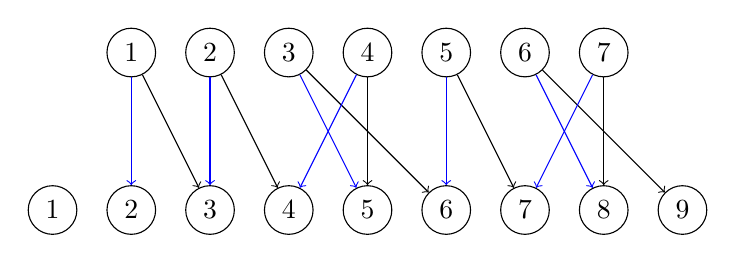
\begin{tikzpicture}              
            \node [circle, draw=black] (J1) at (3, 6) {$1$}; 
            \node [circle, draw=black] (J2) at (4, 6) {$2$}; 
            \node [circle, draw=black] (J3) at (5, 6) {$3$}; 
            \node [circle, draw=black] (J4) at (6, 6) {$4$}; 
            \node [circle, draw=black] (J5) at (7, 6) {$5$}; 
            \node [circle, draw=black] (J6) at (8, 6) {$6$}; 
            \node [circle, draw=black] (J7) at (9, 6) {$7$}; 
            
            \node [circle, draw=black] (T1) at (2, 4) {$1$}; 
            \node [circle, draw=black] (T2) at (3, 4) {$2$}; 
            \node [circle, draw=black] (T3) at (4, 4) {$3$}; 
            \node [circle, draw=black] (T4) at (5, 4) {$4$}; 
            \node [circle, draw=black] (T5) at (6, 4) {$5$}; 
            \node [circle, draw=black] (T6) at (7, 4) {$6$}; 
            \node [circle, draw=black] (T7) at (8, 4) {$7$}; 
            \node [circle, draw=black] (T8) at (9, 4) {$8$}; 
            \node [circle, draw=black] (T9) at (10, 4) {$9$};
            
            \draw [->, color=blue] (J1) -- (T2); \draw [->] (J1) -- (T3); 
            \draw [->, color=blue] (J2) -- (T3); \draw [->] (J2) -- (T4); 
            \draw [->, color=blue] (J3) -- (T5); \draw [->] (J3) -- (T6);
            \draw [->, color=blue] (J4) -- (T4); \draw [->] (J4) -- (T5); 
            \draw [->, color=blue] (J5) -- (T6); \draw [->] (J5) -- (T7); 
            \draw [->, color=blue] (J6) -- (T8); \draw [->] (J6) -- (T9); 
            \draw [->, color=blue] (J7) -- (T7); \draw [->] (J7) -- (T8); 
        \end{tikzpicture} 
    \end{center}
    \begin{center}
        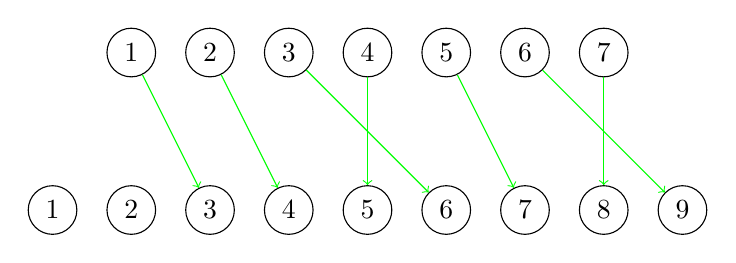
\begin{tikzpicture}              
            \node [circle, draw=black] (J1) at (3, 6) {$1$}; 
            \node [circle, draw=black] (J2) at (4, 6) {$2$}; 
            \node [circle, draw=black] (J3) at (5, 6) {$3$}; 
            \node [circle, draw=black] (J4) at (6, 6) {$4$}; 
            \node [circle, draw=black] (J5) at (7, 6) {$5$}; 
            \node [circle, draw=black] (J6) at (8, 6) {$6$}; 
            \node [circle, draw=black] (J7) at (9, 6) {$7$}; 
            
            \node [circle, draw=black] (T1) at (2, 4) {$1$}; 
            \node [circle, draw=black] (T2) at (3, 4) {$2$}; 
            \node [circle, draw=black] (T3) at (4, 4) {$3$}; 
            \node [circle, draw=black] (T4) at (5, 4) {$4$}; 
            \node [circle, draw=black] (T5) at (6, 4) {$5$}; 
            \node [circle, draw=black] (T6) at (7, 4) {$6$}; 
            \node [circle, draw=black] (T7) at (8, 4) {$7$}; 
            \node [circle, draw=black] (T8) at (9, 4) {$8$}; 
            \node [circle, draw=black] (T9) at (10, 4) {$9$};
            
            \draw [->, color=green] (J1) -- (T3); 
            \draw [->, color=green] (J2) -- (T4); 
            \draw [->, color=green] (J3) -- (T6);
            \draw [->, color=green] (J4) -- (T5); 
            \draw [->, color=green] (J5) -- (T7); 
            \draw [->, color=green] (J6) -- (T9); 
            \draw [->, color=green] (J7) -- (T8); 
        \end{tikzpicture} 
    \end{center}
    Letting red denote machine $1$, blue denote machine $2$, and 
    green denote machine $3$, we are led to the following schedule
    which has $L_{\max} = 1$. 
    \begin{center} 
        \begin{tikzpicture}[/pgfgantt/y unit chart=0.7cm] 
            \begin{ganttchart}[
                title/.style={draw=none},
                canvas/.append style={draw=none}, 
                bar top shift=0.1, bar height=0.6,
                y unit title=0.7cm,
            ]{1}{9}
                \ganttbar{Machine 1}{1}{1} \ganttbar[inline]{1}{1}{1} \ganttbar[inline]{2}{2}{2} 
                \ganttbar[inline]{3}{4}{4} \ganttbar[inline]{5}{5}{5} \ganttbar[inline]{4}{6}{6} 
                \ganttbar[inline]{6}{7}{7} \ganttbar[inline]{7}{9}{9} \\ 
                \ganttbar{Machine 2}{2}{2} \ganttbar[inline]{1}{2}{2} \ganttbar[inline]{2}{3}{3}
                \ganttbar[inline]{4}{4}{4} \ganttbar[inline]{3}{5}{5} \ganttbar[inline]{5}{6}{6} 
                \ganttbar[inline]{7}{7}{7} \ganttbar[inline]{6}{8}{8} \\ 
                \ganttbar{Machine 3}{3}{3} \ganttbar[inline]{1}{3}{3} \ganttbar[inline]{2}{4}{4} 
                \ganttbar[inline]{4}{5}{5} \ganttbar[inline]{3}{6}{6} \ganttbar[inline]{5}{7}{7} 
                \ganttbar[inline]{7}{8}{8} \ganttbar[inline]{6}{9}{9} \\ 
                \gantttitlelist{1,...,9}{1} 
            \end{ganttchart}
        \end{tikzpicture}
    \end{center}
    \vspace{-0.4cm}
    Note that we have not verified at this point whether or not there is a 
    feasible schedule for $L = 0$. But by running this algorithm again 
    with this parameter, we can find a certificate of infeasibility 
    for the network flow problem. For example, one could determine 
    the dual of the transportation model we discussed above and show 
    that the dual is unbounded, which implies that the transportation 
    model is infeasible. Thus, there does not exist a schedule 
    in which every job is completed on time.
\end{exmp}